%\documentclass[a4paper,11pt]{report}
\documentclass[a4paper,11pt]{article}
\usepackage[utf8]{inputenc}
\usepackage[italian]{babel}
\usepackage{amsmath,amssymb, enumerate, indentfirst, booktabs, listings, colortbl, tabularx, graphicx, url}
\usepackage{emp} 

% include the web pages examined in the bibliography
\makeatletter
\let\@orig@endthebibliography\endthebibliography
\renewcommand\endthebibliography{
\xdef\@kept@last@number{\the\c@enumiv}
\@orig@endthebibliography}
\newenvironment{thesitography}[1]
%{\def\bibname{Siti consultati}% Classe book o report
{\def\refname{Siti consultati}% Classe article
\thebibliography{#1}%
\setcounter{enumiv}{\@kept@last@number}%
}
	{\@orig@endthebibliography}
\makeatother

\definecolor{orange}{rgb}{1,0.5,0}
\lstnewenvironment{java}{\lstset{basicstyle=\ttfamily,
stepnumber=2, numbersep=5pt, language=java, %frame=shadowbox, 
keywordstyle=\color{red}\bfseries, commentstyle=\color{blue}, 
stringstyle=\color{orange}}}{}

\newcolumntype{G}{>{\columncolor[gray]{0.8}}c}

\setlength{\parindent}{3mm}
\newcommand{\grammarindent}[1][1]{\hspace*{#1\parindent}\ignorespaces} 


% set margin
\usepackage{vmargin}
\setpapersize{A4}
\setmarginsrb{25mm}{5mm}{25mm}{8mm}
             {0mm}{10mm}{0mm}{10mm}


\title{\bf{Implementazione di un dimostratore di teoremi per risoluzione}}
\author{Enrico Scapin vr353597}
\date{\today}

\begin{document}

\maketitle

\section{Introduzione}
Uno degli obiettivi del ragionamento automatico consiste nel cercare di costruire \emph{Dimostratori Automatici di Teoremi} al fine di ottenere meccanismi automatizzabili per asserire, a partire da un insieme di assunzioni $H$, la validità o meno di una determinata congettura $\varphi$. Più formalmente:
\[ H \models \varphi \]
I dimostratori automatici tipicamente procedono in maniera refutazionale in quanto ogni formula è valida se e solo se la sua negazione è insoddisfacibile. Quindi, riferendoci al sequente sopra:
\[ H \models \varphi \Longleftrightarrow H \cup \lbrace\neg \varphi\rbrace \text{ è insoddisfacibile} \]
Da questa considerazione possiamo quindi cercare di costruire una procedura che, se dimostra l'insoddisfacibilità di $H \cup \lbrace\neg \varphi\rbrace$, allora $ H \models \varphi $ è valido, altrimenti, se ne dimostra la sua soddisfacibilità, il modello che lo soddisfa costituirà il controesempio alla validità di $ H \models \varphi $.\par
Siamo interessati a dimostrare formule espresse in Logica del Primo Ordine\footnote{\emph{FOL}, First Order Logic} in quanto, al contrario della logica proposizionale, essa è sufficientemente espressiva da poter modellare una buona parte della nostra conoscenza. Utilizzando questo linguaggio però il problema della validità non è più decidibile bensì semidecidibile: infatti se l'insieme $H \cup \lbrace\neg \varphi\rbrace $ è insoddisfacibile allora è possibile costruire una procedura che termina, mentre se esso è soddisfacibile non è detto che termini. \par
La semidecidibilità deriva direttamente dal \emph{Teorema di Herbrand} che afferma che un insieme finito $S$ di clausole in \emph{FOL} è soddisfacibile se e solo se esiste un insieme finito $S'$ di istanze ground (clausole in cui tutte le variabili sono istanziate ad una qualche costante) di clausole di $S$ tale che $S'$ è soddisfacibile. Quindi per dimostrare la soddisfacibilità di $S$ è necessario generare tutti gli insiemi $S'$ di istanze ground e dimostrarne la soddisfacibilità ma, se in $S$ si quantifica su insiemi infiniti, allora la cardinalità degli insiemi $S'$ da generare è anch'essa infinita.\par
Questo dimostratore prende in ingresso un insieme di clausole scritte in Forma Normale Congiunta\footnote{\emph{CNF}, Conjunctive Normal Form} e definite da una sintassi standard compatibile con frammento CNF senza uguaglianza della libreria \emph{TPTP} (vedi \cite{TPTP}). Si è quindi implementata una procedura di semi-decisione che, basata su un sistema di cinque regole di inferenza (di cui due di espansione e tre di contrazione), implementa un piano di ricerca denominato \emph{Ciclo della Clausola Data} (Given clause loop) che è uno standard alla base di molti dimostratori di insieme di formule in logica al primo ordine come Otter, E, Vampire etc.

%%%%%% Scelte progettuali implementative %%%%%%%%
\section{Scelte progettuali ed implementative}
L'elaborato è stato implementato utilizzando il linguaggio \emph{Java} in quanto il livello di astrazione è tale da permettere al programmatore di concentrarsi principalmente sulla progettazione dell'algoritmo ed, in particolare, su quali strutture dati sia meglio utilizzare. 
\subsection{Parser}
La scelta di \emph{Java} consente l'utilizzo di \emph{JavaCC}, uno strumento che permette di effettuare sia il parsing delle formule sia quello degli argomenti che vengono passati da riga di comando: i due parser consistono in file con estensione \texttt{.jj} costituiti da un'unità di compilazione java e da una grammatica context-free di tipo \emph{LL(1)} le cui produzioni sono espresse in BNF (\emph{Backus–Naur Form}).
Per quanto riguarda il parsing degli argomenti la grammatica è molto semplice:
\\[1mm]
\begin{ttfamily}
\grammarindent SelectionStrategy $::=$  -fifo | -best$($<Numeric>$)?$ \\
\grammarindent SearchStrategy ~~~$::=$  -contr | -exp \\
\grammarindent LoopType $::=$ 	-o | -e\\
\grammarindent Time ~~~~$::=$ 	-time<Numeric>\\
\grammarindent FilePath $::=$ <Char>\\
\\[1mm]
\end{ttfamily}
I token \texttt{<Numeric>} e \texttt{<Char>} sono specificati dalle 
seguenti espressioni regolari:\\[1mm]
\begin{ttfamily}
\grammarindent Numeric $::=$ $($["0"-"9"]$)^+$\\
\grammarindent Char~~~ $::=$ $\widehat{}$["-","\textbackslash t"]$($ $\widehat{}$["\textbackslash t"]$)^*$\\[1.5mm]
\end{ttfamily}
Queste categorie indicano le possibilità con coi può essere eseguito il dimostratore implementato e sono documentate nel file README: si è deciso di utilizzare il parser per dare all'utente la possibilità di inserirli nell'ordine preferito ed inoltre solo il token \texttt{FilePath} è obbligatorio (in quanto consiste nella formula in input che deve essere dimostratata).
La configurazione di default degli argomenti in cui è prevista una scelta è la seguente:\\[1mm]
\begin{ttfamily}
\grammarindent SelectionStrategy $::=$  -best \\
\grammarindent SearchStrategy ~~~$::=$  -contr\\
\grammarindent LoopType $::=$ 	-o \\
\\[1mm]
\end{ttfamily}
Il significato semantico di ognuno di essi sarà spiegato successivamente.\par 
Per quanto riguarda invece il parsing del file contentente le formule, la grammatica corrisponde al frammento \emph{CNF} senza uguaglianza di quella di TPTP che può essere reperita in \cite{TPTPsyntax}. Per ogni categoria sintattica stato inserito del codice Java che si preoccupa di costruire ciascuna clausola, partendo dai suoi letterali (e a loro volta dai loro termini), per poi inserirla nella struttura dati apposita. Il tipo di struttura dati dipende dall'argomento inserito dall'utente per il token \texttt{SelectionStrategy}: nel caso sia stato inserito \texttt{-best} la struttura dati è una coda di min priorità in cui l'ordinamento è definito dal numero di simboli presenti in ciascuna clausola, altrimenti nel caso sia stato inserito \texttt{-fifo} la struttura dati è una lista in cui le clausole vengono inserite nell'ordine in cui vengono lette.

\subsection{Bean Class}
La scelta dell'utilizzo di \emph{Java} ha anche permesso un minimo di progettazione orientata agli oggetti soprattutto delle cosidette classi bean\footnote{così si denotano le classi che logicamente contengono le informazioni da manipolare} e, in particolare, delle classi che definisco i termini (funzioni, variabili e costanti) e i letterali. 

\begin{figure}[h]
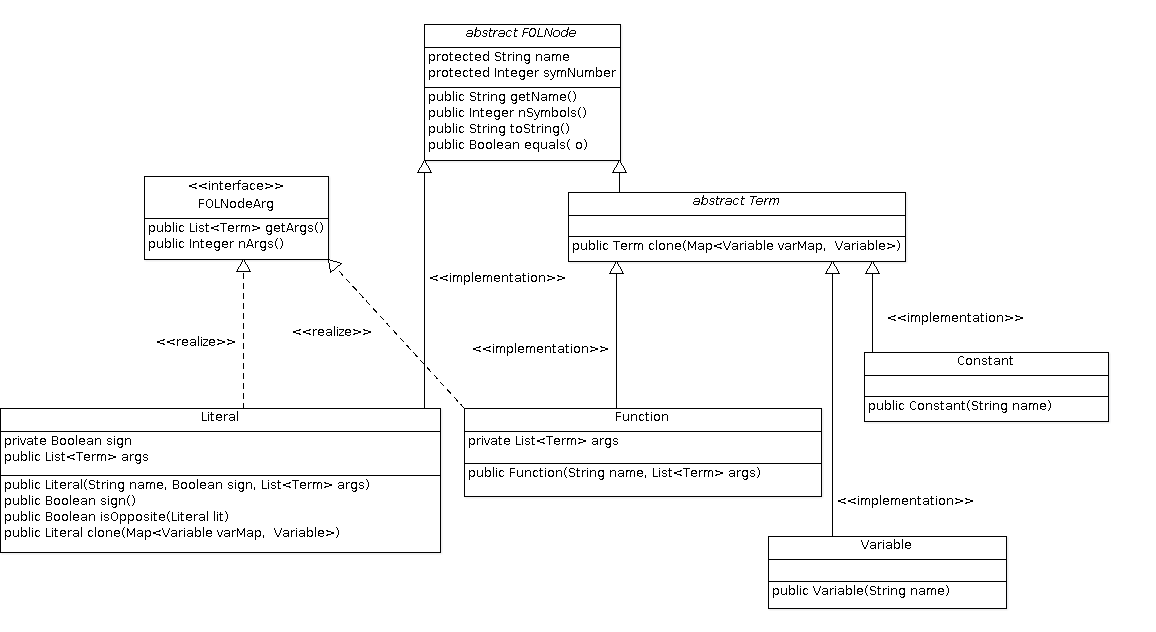
\includegraphics[width=1\columnwidth]{beanClassUML}
\caption{\small{UML delle bean class}}
\label{beanClassUML}
\end{figure}

Il diagramma UML visibile in Figura \ref{beanClassUML} rappresenta come è state progettate le classi: molto rilevante la classe astratta \texttt{Term}, che è superclasse di \texttt{Function}, \texttt{Variable} o \texttt{Constant}, poiché è spesso necessario riferirsi alla classe che le rappresenta tutte (come ad esempio quando si specificano gli argomenti di un letterale). \par
Il metodo \texttt{clone(Map<Variable, Variable>)} presente sia nella classe \texttt{Term} sia nella classe \texttt{Literal} permette di clonare l'oggetto in questione restituendone un altro con la stessa struttura. Questo metodo si rivela essere molto importante quando è necessario generare una nuova clausola a partire da un'altra: infatti è sufficiente chiamare il metodo \texttt{clone} su ogni letterale che ricorsivamente clonerà anche i termini che compongono i suoi argomenti. Quando si crea un nuova clausola è però necessario mantenere inalterato il numero delle variabili in modo tale che tutte le occorrenze di ogni variabile nella vecchia clausola vengano rimpiazzate dalla stessa nuova variabile nella nuova. Per far ciò è necessaria una mappa che mantenga il collegamento tra il vecchio e il nuovo oggetto \texttt{Variable}: se la variabile è stata già creata in precedenza in quanto presente in un altro termine non deve di nuovo venire ricreata per cui il metodo restituirà la stessa,  alternativamente se quella variabile non è presente nella struttura dati allora è necessario crearne una nuova e inserire la coppia $(vecchia, nuova)$ all'interno della mappa.\par
Per quanto riguarda il metodo \texttt{toString} è da segnalare l'implementazione nella classe \texttt{Variable} in quanto, per differenziare le variabili diverse ma con lo stesso simbolo, si è scelto di concatenarci gli ultimi 3 caratteri del loro \emph{hash code} codificato in esadecimale.\par
Da notare infine il metodo \texttt{equals} che per quanto riguarda le variabili ritorna \texttt{true} se e solo se sono lo stesso oggetto mentre per quanto riguarda le costanti se esse sono rappresentate dallo stesso simbolo (e questo è consistente col fatto che le costanti sono le stesse per tutto l'insieme di clausole). Di conseguenza i metodi \texttt{equals} delle funzioni e dei letterali, dopo aver controllato l'uguaglianza dei segni e/o dei nomi, vanno in ricorsione sui termini che compongono i loro argomenti e, solo se sono tutti uguali, ritornano \texttt{true}.

\subsection{Core Class}
Le classi contenute nel package \emph{core} sono quelle responsabili della parte computazionale.
\subsubsection{Unifier}
La classe Unifier contiene i metodi \texttt{findMGU} e \texttt{findLeftSubst} che, date due liste di argomenti, restituiscono il primo l'unificatore più generale\footnote{\emph{MGU}, Most General Unifier} tra le due liste mentre il secondo una sostituzione che, se applicata alla prima lista di argomenti, li rende sintatticamente identici alla seconda lista. In entrambi i casi essi restitutisco una \texttt{HashMap} formata da coppie \texttt{<Variable, Term>} se l'\emph{MGU} o la sostituzione esiste, altrimenti \texttt{null}. Per quanto riguarda l'\emph{MGU} si è deciso di implementare l'algoritmo presente nel libro \emph{Artificial Intelligence: A Modern Approach} (vedi \cite{AIMAbook} e \cite{AIMAalgo}) che è quadratico nella grandezza delle espressioni che devono essere unificate. A questo algoritmo è stato aggiunto un metodo chiamato \texttt{cascadeSubst} che rende la sostituzione idempotente, ovvero tutte le variabili presenti nel suo range e che fanno anche parte del suo dominio vengono sostituite con il corrispettivo termine.
\subsubsection{Substitution}
La classe Substitution si occupa data una sostituzione di applicarla ad un letterale o ad un termine. Questi metodi ritornano sempre un nuovo oggetto e non il vecchio a cui è stata applicata la sostituzione in quanto in tutte le regole di inferenza ogni volta che si applica una sostituzione è per generare una nuova clausola che quindi dovrà avere nuovi letterali e termini. Proprio per questa ragione in questa classe si fa ingente uso del metodo \texttt{clone} spiegato precedentemente.
\subsubsection{ExpansionRules}
La classe ExpansionRules implementa le due regole di espansione Risoluzione Binaria e Fattorizzazione entrambe in due modalità differenti: nella prima vengono passate solamente la (o le) clausole e si cerca di generare tutti i fattori (o i risolutori binari) restituendo un oggetto di tipo \texttt{Collection} con tutte le nuove clausole generate, mentre nella seconda vengono anche passati i due letterali e la regola di inferenza viene applicata una sola volta su di essi. Entrambe le procedure consistono nella verifica della compatibilità tra i due letterali (simbolo e segno) e, in caso positivo, nella ricerca di \emph{MGU} tra le due liste dei loro termini e, se questo viene trovato, nella creazione di un nuovo fattore o risolvente binario. A tale scopo sono presenti anche due metodo \texttt{createFactor} e \texttt{createResolvent} che, chiamando i metodi della classe \texttt{Substitution}, generano una nuova clausola.
\subsubsection{Clause}
La classe Clause, oltre a contenere i metodi per l'aggiunta dei letterali che la compongono, implementa anche le tre regole di contrazione: eliminazione delle tautologie, semplificazione clausale e sussunzione.\par
Per quanto riguarda l'eliminazione delle tautologie, il metodo \texttt{isTautology} cerca due letterali che siano opposti ovvero che abbiano stesso simbolo, stessi argomenti ma segno opposto: solo in caso positivo questo metodo ritorna \texttt{true}.\par
Per quanto riguarda la semplificazione clausale, il metodo \texttt{simplify} prende come argomento un'altra clausola che prova a semplificarla. Per prima cosa si controlla che la clausola inserita abbia un unico letterale, in caso positivo per ogni letterale compatibile nella clausola chiamante si cerca una sostituzione (tramite il metodo \texttt{findLeftSubst}) da applicare al letterale della clausola inserita in modo che divenga sintatticamente uguale al letterale selezionato; in caso affermativo si elimina dalla clausola chiamate tale letterale. Un'euristica implementata è che questo procedimento non si fermi al primo letterale eliminato ma continui cercando di semplificare più letterali possibile. I letterali eliminati vengono ritornati tramite un oggetto di tipo \texttt{Collection}.\par
Per quanto riguarda la sussunzione, di gran lunga la regola di inferenza più onerosa dal punto di vista computazionale, il metodo \texttt{subsumes} controlla se la clausola chiamate sussume la clausola inserita come argomento. Tale metodo implementa l'algoritmo presente nel libro \emph{Symbolic Logic and Mechanical Theorem Proving} (vedi \cite{ChangLee}) con qualche euristica. Infatti condizioni necessarie per cui una clausola ne sussuma un'altra sono:
\begin{itemize}
\item il numero di letterali della clausola che sussume deve essere minore o uguale al numero di letterali della clausola da sussumere;
\item il numero di simboli della clausola che sussume deve essere minore o uguale al numero di simboli della clausola da sussumere: questa condizione è stata dimostrata nel paper \emph{Towards Efficient Subsumption} (vedi \cite{efficientSubsum});
\item per ogni letterale nella clausola che sussume vi deve essere almeno un letterale nella clausola da sussumere con lo stesso simbolo e stesso segno.
\end{itemize}
Solo se queste tre condizioni sono soddisfatte si procede con l'algoritmo di sussunzione che però è una versione modificata rispetto a quella del libro di testo. Si mantiene sempre l'insieme delle clausole generate $U$ e si termina restituendo \texttt{true} se viene trovata la clausola vuota, \texttt{false} se invece quest'insieme si svuota. Ciò che cambia è come vengono generate le clausole che ad ogni iterazione vengono inserite in $U$:
\begin{enumerate}
\item per ogni clausola in $U$ e per ogni letterale di questa clausola viene eseguito il metodo \texttt{findLeftSubst} tra i suoi argomenti e quelli di un letterale della clausola inserita come argomento;
\item in caso si trovi una sostituzione si crea una nuova clausola a partire da quella che era in $U$ a cui si applica la sostituzione senza considerare il letterale che, istanziato, è sintatticamente equivalente a quello nella clausola inserita come argomento (da notare che ciò è effettuato semplicemente chiamando il metodo \texttt{createFactor});
\item una volta generati tutte le nuove clausole l'insieme $U$ viene svuotato e ripopolato con le nuove clausole generate a tale iterazione.
\end{enumerate}

\subsection{Strategia di ricerca}
Il Strategia di Ricerca consiste nella parte algoritmica che decide a quali clausole applicare le cinque regole di inferenza e si basa principalmente sull'algoritmo della clausola data. Sono state implementate due versioni di tale algoritmo: il ciclo à la \emph{Otter}, selezionabile tramite il comando \texttt{-o}, e il ciclo à la \emph{E}, selezionabile tramite il comando \texttt{-e}. \par
In entrambi si lavora con due insiemi di clausole: \texttt{toBeSelected}, che all'inizio contiene le clausole in input e da cui viene prelevata la clausola data secondo un criterio di peso o di inserimento, e \texttt{alreadySelected} che contiene le clausole già selezionate che servono principalmente per cercare di generare nuove clausole tramite l'applicazione della regola di risoluzione binaria. Una volta generate le nuove clausole, le regole di contrazione devono essere applicate in maniera \texttt{eagerly} per evitare di generare clausole da clausole che potevano essere cancellate per contrazione. Le due versioni differiscono nell'implementazione della strategia di contrazione: \emph{Otter} cerca di mantenere l'unione di \texttt{toBeSelected} e \texttt{alreadySelected} inter-ridotto mentre \emph{E} cerca di mantenere inter-ridotto solamente \texttt{alreadySelected}.\par 
Alla fine di ogni iterazione le nuove clausole generate verranno inserite in \texttt{toBeSelected} in attesa di divenire \emph{given-clause}. Non appena una regola di inferenza (risoluzione binaria o semplificazione clausale) genera la clausola vuota si esce dal ciclo restituendo UNSAT. Se invece \texttt{toBeSelected} si svuota allora l'insieme di clausole in ingresso è soddisfacibile per cui viene ritornato SAT. \par
Per quanto riguarda la generazione di nuove clausole mediante regole di espansione sono state individuate due strategie: 
la prima consiste, ogni volta che una nuova clausola è stata generata tramite una regola di espansione, di cercare di applicare una qualche regola di contrazione con \texttt{alreadySelected} e, nel caso del ciclo à la Otter, anche con \texttt{toBeSelected}; la seconda invece consiste nel generare prima tutte le clausole tramite regole di espansione (fattorizzazione e risoluzione binaria) poi rendere inter-ridotto questo insieme di nuove clausole ed infine per ogni clausola rimasta, cercare di inter-ridurre \texttt{alreadySelected} e, in caso di ciclo à la Otter, anche \texttt{toBeSelected}. Le due possibilità sono selezionabili rispettivamente tramite i comandi \texttt{-contr} e \texttt{-exp}.\par
Per quanto riguarda invece l'applicazione delle regole di contrazione, se una clasuola è tautologica oppure è sussunta da un'altra deve essere eliminata dall'insieme di appartenenza mentre, se viene semplificata, deve essere prelevata da tale insieme e trattata come se fosse una nuova clausola generata.\par
L'ultimo aspetto rilevante della strategia di ricerca consiste, nel caso la clausola venga prelevata tramite una strategia \emph{Best Visit First}, di poter opzionalmente inserire anche il \emph{Peak Given Ratio}, che ogni \texttt{k}\footnote{di solito il \emph{Peak Given Ratio} è compreso tra 4 e 6} iterazioni preleva non la clasuola con peso minore, ma quella che da più tempo è in \texttt{toBeSelected} (si passa quindi ad una strategia FIFO). Per far ciò viene mantenuta una struttura dati parallela di tipo \texttt{LinkedHashSet} che contiene tutte le clausole secondo l'ordine di inserimento permettendo quindi ogni \texttt{k} iterazioni di selezionare la clausola che da più tempo si trova nell'insieme.

\section{Benchmark}
In questa sezione viene riportata l'analisi delle prestazioni di tale metodo effettuata su un calcolatore con CPU \texttt{Intel Core 2 Duo P8600 2.4GHz}, sistema operativo \texttt{Ubuntu 11.10} e \texttt{JVM v1.6.0\_26}.\\
Da notare che uno degli argomenti che possono essere inseriti è \texttt{-time} seguito da un numero che indica il limite massimo di secondi entro cui il ciclo della clausola data può cercare una prova di insoddisfacibilità o un modello per la soddisfacibilità. Ovviamente nel caso questo parametro non sia specificato il tempo di esecuzione rimante potenzialmente infinito. Inoltre se il numero di clausole generate per regole di espansione siano tali da eccedere l'heap space della \emph{thread} (appositamente creata per eseguire il ciclo), allora essa viene chiusa e la risposta sarà \emph{out of memory}.\par
Sono presentate due tabelle con alcuni dei dati raccolti sulle prestazioni dell'algoritmo con un timeout di 300 secondi e  strategia di selezione della clausola data di tipo \emph{Best Visit First}.

\begin{table}[!htp]
\center
\begin{tabular}{lGcccc}
\toprule
File & Status & Otter contr & Otter exp &  E contr & E exp \\
\midrule
ALG002-1 & UNSAT & 445 & 2523 & 4695 & 3174 \\
ANA002-1 & UNSAT & 12266 & 13106 & 27285 & 62456 \\
ANA004-5 & UNSAT & 6410 & 6410 & 6828 & 6410 \\
CAT007-3 & UNSAT & 245 & 260 & 561 & 260 \\
KRS006-1 & SAT & 61311 & time expired	& time expired	& time expired	\\
NUM284-1.014 & UNSAT & 3610 & out of memory & 11509	& out of memory	\\ 
PUZ001-3 & SAT & 148 & 152 & 305 & 160\\
PUZ012-1 & UNSAT & 234 & 239 & 467 & 250 \\
PUZ018-1 & UNSAT & time expired & out of memory & time expired & out of memory \\
SYN086-1.003 & SAT & 757 & 813 & 8393 & 813 \\
SYN087-1.003 & SAT & 2583 & 2621 & 66101 & 2621 \\
\bottomrule
\end{tabular}
\caption{Numero di clausole generate dalle regole di espansione}
\end{table}

\begin{table}[!htp]
\center
\begin{tabular}{lcccc}
\toprule
File & Otter contr (ms) & Otter exp (ms) &  E contr (ms) & E exp (ms) \\
\midrule
ALG002-1 & 981 & 2833 & 3537 & 2793 \\
ANA002-1 & 8735 & 9354 & 16938 & 32813 \\
ANA004-5 & 42079 & 45167 & 16853 & 14107 \\
CAT007-3 & 141 & 216 & 278 & 230\\
KRS006-1 & 123598 &	time expired & time expired	& time expired	\\
NUM284-1.014 & 30398 & out of memory & 33460 & out of memory	\\
PUZ001-3 & 120 & 146 & 199 & 159\\
PUZ012-1 & 196 & 325 & 606 & 351 \\
PUZ018-1 & time expired & out of memory & time expired & out of memory \\
SYN086-1.003 & 365 & 393 & 1477 & 439 \\
SYN087-1.003 & 1392 & 2489 & 7287 & 2594 \\
\bottomrule
\end{tabular}
\caption{Tempistiche a seconda della strategia}
\end{table}
\subsection{Considerazioni}
Nelle due tabelle è possibile osservare rispettivamente il numero di clausole generate dalle regole di espansione e i tempi di esecuzione a seconda della strategia di ricerca. Nella cartella \texttt{test/} per ogni insieme di clausole testato è presente un altro file con tutte le altre statistiche qui omesse.
Dalla prima tabella si può notare come l'implementazione di \emph{E} in genere genera più clausole prima di restituire la risposta corretta: questo perché \emph{E} non mantiene \texttt{toBeSelected} inter-ridotto e quindi se la \emph{given clause} che genera la clausola vuota ha un rating alto verrà prelevata successivamente generando nel frattempo molte altre clausole. Di conseguenza, nonostante in \emph{E} vengano eseguite meno regole di contrazione, i tempi sono leggermente maggiori: molto probabilmente i tempi in \emph{E} si avvicinerebbero maggiormente a quelli di \emph{Otter} se non fossero state implementate le euristiche sulla regola di sussunzione (il vero responsabile del decreasing delle prestazioni) in quanto il vantaggio di non applicare eccessivamente le regole di contrazione sarebbe equiparabile al vantaggio di mantenere entrambi gli insiemi inter-ridotti. A favore di questa tesi è stato riportato l'esempio ANA004-5 nel quale \emph{Otter} impiega più tempo di \emph{E}: ciò accade proprio a causa dell'applicazione delle regole di contrazione tra le clausole generate e \texttt{toBeSelected} in cui evidentemente si esegue in modo massiccio l'algoritmo di sussunzione.\par
Per quanto riguarda invece la scelta se prima applicare tutte le regole di espansione e poi contrarre oppure cercare di contrarre ogni clausola appena generata, sembra che quest'ultima strategia sia più efficiente ed, in taluni casi (e.g. KRS006-1), permetta l'uscita dal ciclo che invece deve essere interrotto con risultato \emph{time expired} o \emph{out of memory} in caso si adotti l'altra strategia. A tal proposito emblematico è il problema PUZ018-1 che se eseguito col comando \texttt{-contr} non termina a causa del tempo scaduto mentre con \texttt{-exp} a causa dell'eccessiva memoria allocata.

\begin{thebibliography}{9}
\bibitem{ChangLee} 	Chang~C.L. Lee~R.C.T. (1973),	
\newblock "Symbolic Logic and Mechanical Theorem Proving", \emph{Academic Press}.
\bibitem{AIMAbook} Russell~S. Norvig~P. (2010),
\newblock "Artificial Intelligence: A Modern Approach (Third Edition)", \emph{Prentice Hall}.
\bibitem{efficientSubsum} Tammet T. (1998),
\newblock "Towards Efficient Subsumption", \emph{Lecture Notes in Computer Science. Springer Verlag}. 
\end{thebibliography}
\begin{thesitography}{9}
\bibitem{TPTP}
\url{http://www.cs.miami.edu/~tptp/}
\bibitem{TPTPsyntax}
\url{http://www.cs.miami.edu/~tptp/TPTP/SyntaxBNF.html}		
\bibitem{AIMAalgo}
\url{http://aima.cs.berkeley.edu/algorithms.pdf}
\end{thesitography}

\end{document}
